\documentclass[conference]{IEEEtran}
\IEEEoverridecommandlockouts
\usepackage{cite}
\usepackage{amsmath,amssymb,amsfonts}
\usepackage{graphicx}
\usepackage{textcomp}
\usepackage{xcolor}
\usepackage{booktabs}
\usepackage{array}
\usepackage{caption}

\begin{document}

\title{Explainable Machine Learning for Repository Health Assessment in Software Governance: A Comparative Study Using SHAP}

\author{
\IEEEauthorblockN{FIRST AUTHOR NAME\IEEEauthorrefmark{1}, SECOND AUTHOR NAME\IEEEauthorrefmark{2}}
\IEEEauthorblockA{\IEEEauthorrefmark{1}Department of Computer Science and Engineering, INSTITUTION NAME, CITY, COUNTRY \\
email@example.edu}
\IEEEauthorblockA{\IEEEauthorrefmark{2}Department/Role, INSTITUTION NAME, CITY, COUNTRY \\
email@example.edu}
}

\maketitle

\begin{abstract}
Software repository governance tools increasingly rely on automated scoring mechanisms to
flag at-risk projects, yet most existing tools reduce complex activity signals into a
single opaque score without exposing the reasoning behind it. This paper investigates
whether a repository's governance health classification can be predicted from raw,
independently-collected GitHub activity metrics---star count, issue counts, commit
activity, contributor count, and related indicators---while explicitly avoiding label
leakage from the composite scoring formulas typically used to derive such labels. Four
ensemble classifiers (Decision Tree, Random Forest, Gradient Boosting, XGBoost) were
compared on a dataset of 128 real open-source repositories using stratified 5-fold
cross-validation under realistic class imbalance (86\% Healthy, 9\% Needs Attention, 5\%
Critical). Gradient Boosting achieved the best balanced performance (macro-F1 = 0.659,
accuracy = 0.891). SHapley Additive exPlanations (SHAP) were applied to identify global
feature importance and to generate local explanations, revealing that defect-related
signals---bug-labelled issue count and total open issue count---dominate the model's
predictions, while community-scale metrics such as stars and forks contribute
comparatively little. A case study further demonstrates SHAP's value as a diagnostic tool
for understanding model misclassifications, not solely for building confidence in correct
predictions. These findings offer an empirically grounded, explainable methodology for
software governance risk assessment and highlight specific limitations---small sample
size, heuristic rather than independently validated ground-truth labels, and untested
generalizability to enterprise repositories---that should guide future work in this
direction.
\end{abstract}

\begin{IEEEkeywords}
explainable artificial intelligence, SHAP, software repository analytics, AI governance, project management office, ensemble learning, class imbalance
\end{IEEEkeywords}

\section{Introduction}

Modern open-source and enterprise software projects increasingly rely on repository
platforms such as GitHub to coordinate development activity, track defects, manage
pull requests, and maintain release cycles. As this activity grows in volume and pace,
manually checking whether a repository is in a healthy governance state stops being
practical, so organizations turn to automated scoring instead. The trouble is that most
existing repository health and risk-scoring tools produce a single number or category
label without showing the reasoning behind it. For governance decision-making this is a
real problem: a Project Management Office (PMO) or engineering lead needs to justify why
a repository was flagged, not just accept that it was.

Two bodies of research speak to this problem, but from different angles. AI governance
and PMO governance frameworks have proposed conceptual models for embedding
accountability, ethics, and human oversight into AI-assisted project management
\cite{ref1,ref2,ref3,ref4,ref5,ref6,ref7,ref8,ref9}. These are largely normative --- they
describe what governance should achieve, not how to measure it from data an organization
already has. Separately, explainable machine learning (XAI) research has shown that SHAP
(SHapley Additive exPlanations) can make ensemble models interpretable in domains such as
materials science, effort estimation, and cybersecurity risk assessment
\cite{ref10,ref11,ref12,ref13}. None of this work, however, applies SHAP to software
repository governance specifically.

This paper sits at the intersection of the two threads. It asks whether a repository's
governance health classification --- derived from a composite scoring procedure that
combines issue, defect, and activity signals --- can be recovered from raw,
independently observable GitHub metrics alone (star count, issue counts, commit
activity, contributor count, and related indicators), and whether SHAP can make that
classification process transparent, including in cases where the model gets it wrong.
A methodological point matters here: unlike prior repository analytics work that reports
predictive accuracy without checking where the labels came from, this study deliberately
separates the raw predictive features from the scoring formula that produced the labels
in the first place, so that a trivially recoverable result is not mistaken for genuine
predictive power.

The contributions of this paper are as follows:

\begin{enumerate}
\item An empirical comparison of four ensemble classifiers (Decision Tree, Random Forest,
Gradient Boosting, XGBoost) for predicting repository governance health status from
raw GitHub activity metrics, evaluated using stratified cross-validation under
realistic class imbalance.
\item A SHAP-based global and local explainability analysis identifying which raw
repository signals most strongly drive governance health classification, including
an explicit case study of a model misclassification.
\item A transparent, reproducible methodology that distinguishes genuinely predictive
evaluation from label-formula recovery, addressing a methodological risk that is
often left unexamined in repository analytics literature.
\item A discussion of the practical implications and limitations of applying explainable
ensemble learning to software governance decision support, framed against existing
AI governance and PMO governance literature.
\end{enumerate}

The remainder of this paper is organized as follows. Section II reviews related work in
AI governance, PMO governance, and explainable machine learning. Section III describes
the dataset and methodology. Section IV presents experimental results. Section V
discusses findings and limitations, and Section VI concludes with directions for future
work.

\section{Related Work}

\subsection{AI Governance and PMO Governance Frameworks}

A substantial body of recent literature addresses AI governance at the conceptual and
policy level. Systematic reviews of AI governance frameworks characterize governance
along four dimensions---who governs, what is governed, when governance applies, and how
it is implemented---and highlight persistent gaps in human oversight and ethical
integration across the AI lifecycle \cite{ref1}. Related work on purpose-led AI governance
argues that technical AI readiness is insufficient without explicit organizational
purpose, accountability structures, and continuous human oversight throughout a project's
lifecycle \cite{ref2}. Complementary work embeds AI ethics directly into the enterprise
data lifecycle, proposing governance indicators spanning data quality, explainability,
accountability, and stakeholder feedback \cite{ref3}. At the PMO level, empirical studies
of PMO adoption in large-scale projects identify implementation excellence, change
management, and risk management as the strongest predictors of successful governance
adoption \cite{ref4}, while conceptual frameworks for building PMOs from limited
organizational maturity propose phased governance models spanning recognition, design,
capability-building, and continuous improvement \cite{ref5}. Broader systematic reviews of
AI in project management similarly emphasize predictive analytics, decision support, and
resource optimization as recurring AI application areas, while consistently identifying
explainability and governance integration as open challenges rather than solved problems
\cite{ref6,ref7,ref8,ref9}.

Across this literature, a consistent limitation emerges: governance frameworks are
described normatively, in terms of principles, roles, and lifecycle stages, but are
rarely instantiated as measurable, data-driven assessments grounded in artifacts that
organizations already produce, such as repository activity data.

\subsection{Repository Analytics and Software Risk Prediction}

A separate line of work analyzes software repositories directly to characterize project
health, defect risk, or engineering practice. Large-scale empirical studies of GitHub
issues have examined how developers report and resolve privacy- and
data-protection-related concerns, showing that regulatory events such as the introduction
of the GDPR measurably shifted the volume and nature of related repository activity, and
that issue resolution patterns vary systematically with contributor role \cite{ref14}.
This line of work demonstrates that repository-level signals (issue text, contributor
behavior, resolution patterns) carry meaningful governance-relevant information, but it
does not connect these signals to a quantitative, explainable governance-health
classification of the kind proposed in this paper.

\subsection{Explainable Machine Learning and SHAP-Based Interpretation}

SHAP has been applied across multiple engineering domains to render ensemble model
predictions interpretable. In materials engineering, SHAP has been used to explain
gradient-boosted and transformer-based regression models predicting the mechanical
strength of asphalt concrete, identifying dominant material and mixture-design features
through global and local explanation plots \cite{ref10}. Similar AutoML-plus-SHAP
pipelines have been applied to predict hysteresis behavior in shape-memory alloys,
combining automated model selection with post-hoc explanation to increase engineering
trust in model output \cite{ref11}. In software engineering specifically, SHAP and LIME
have been combined with stacking-blending ensembles to explain software effort
estimation, identifying function-point and requirement-volatility features as dominant
cost drivers while explicitly validating model comparisons using non-parametric
statistical tests \cite{ref12}. Closest in spirit to the present study, XGBoost combined
with SHAP has been used to build an explainable intrusion-detection and cyber-risk
analytics framework for critical infrastructure, explicitly framing model reliability
assessment---not merely predictive accuracy---as a governance requirement for
trustworthy AI-based risk decision support \cite{ref13}.

These studies collectively establish SHAP-based explanation as a mature, cross-domain
methodology for rendering ensemble classifiers interpretable, and specifically motivate
treating model reliability, not just accuracy, as a first-class evaluation criterion.
However, none of these studies apply this methodology to software repository governance
or PMO decision support, which is the specific gap addressed in this paper.

\subsection{Summary of the Gap}

Table \ref{tab:gap} summarizes the positioning of this paper relative to the reviewed
literature. AI and PMO governance frameworks \cite{ref1,ref2,ref3,ref4,ref5,ref6,ref7,ref8,ref9}
provide conceptual grounding for what governance should measure but no operational,
data-driven instantiation. Repository analytics studies \cite{ref14} demonstrate that
repository signals carry governance-relevant information but do not build explainable
predictive models from them. SHAP-based XAI studies \cite{ref10,ref11,ref12,ref13}
establish a rigorous explainability methodology but have not been applied to software
governance. This paper combines these three threads.

\begin{table}[htbp]
\caption{Positioning of This Study Relative to Related Work}
\label{tab:gap}
\centering
\small
\begin{tabular}{p{1.5cm}p{1.1cm}p{1.1cm}p{1.1cm}p{1.3cm}}
\toprule
\textbf{Research Area} & \textbf{Gov. Grounding} & \textbf{Real Repo Data} & \textbf{Model Explain.} & \textbf{Reports Failure} \\
\midrule
AI/PMO Governance \cite{ref1,ref2,ref3,ref4,ref5,ref6,ref7,ref8,ref9} & Yes & No & No & No \\
Repo/GitHub Analytics \cite{ref14} & Partial & Yes & No & No \\
SHAP-XAI (other domains) \cite{ref10,ref11,ref12,ref13} & No & No & Yes & Partial \\
\textbf{This Study} & \textbf{Yes} & \textbf{Yes} & \textbf{Yes} & \textbf{Yes} \\
\bottomrule
\end{tabular}
\end{table}

\section{Methodology}

\subsection{System Context}

The experiment builds on data collected by an existing repository governance
dashboard, which pulls activity metrics from the GitHub REST API, stores them in a
SQLite history table, computes rule-based risk, compliance, and health scores, and
renders results through a dashboard and a generated PDF report (Fig.~\ref{fig:context}).
The classifier and explainability layer described in this paper sit downstream of that
pipeline; they consume its stored historical records as the source dataset rather than
altering how data is collected in the first place.

\begin{figure}[htbp]
\centering
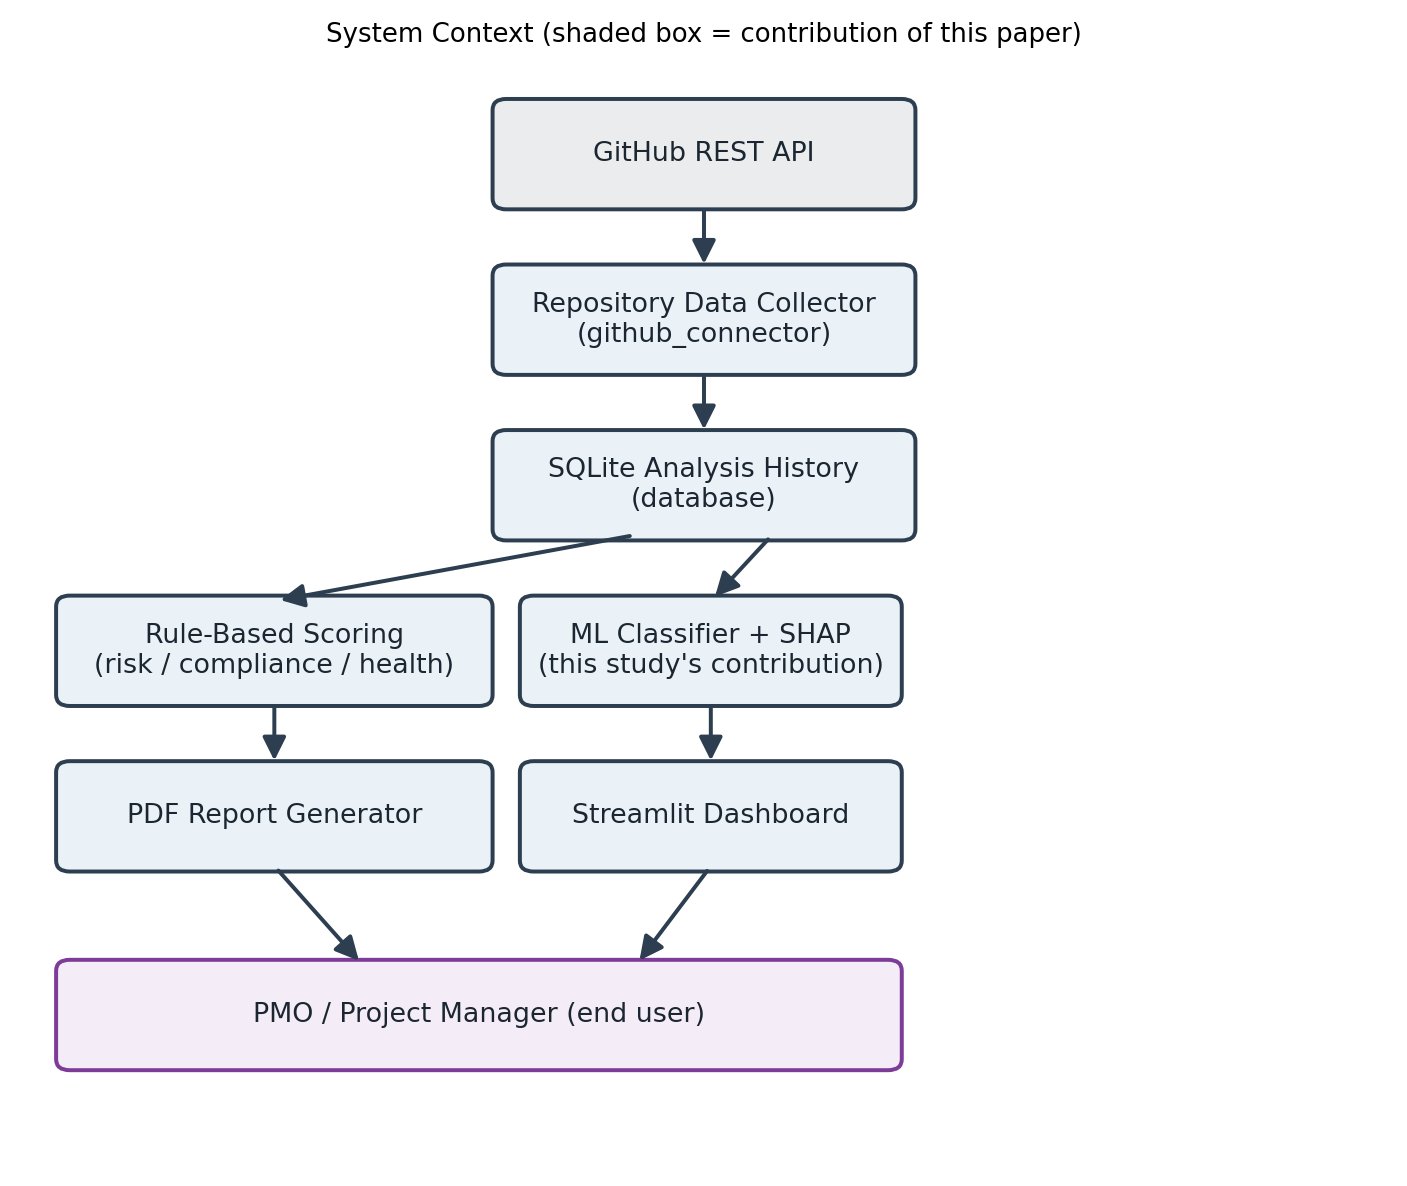
\includegraphics[width=0.85\columnwidth]{figure3_system_context.png}
\caption{System context. The shaded stage is the contribution of this paper; the remaining components already existed in the underlying dashboard tool.}
\label{fig:context}
\end{figure}

\subsection{Dataset}

The study uses a dataset of 128 real, publicly available open-source GitHub repositories
spanning a range of project types, sizes, and maturity levels (e.g., kubernetes, django,
langchain, ansible, terraform, ggplot2). For each repository, the following raw
attributes were collected from the GitHub API: star count, fork count, watcher count,
open issue count, bug-labelled issue count, security-labelled issue count, open pull
request count, recent commit count, release count, contributor count, repository age in
days, and days since the last push.

\subsection{Target Variable and Leakage Prevention}

The prediction target is repository \textbf{health status}, split into three classes:
\textit{Healthy} ($n=110$), \textit{Needs Attention} ($n=12$), and \textit{Critical}
($n=6$), shown in Fig.~\ref{fig:dist}. This label comes from a composite scoring
procedure that combines a risk score, a compliance score, and recent commit activity.

To avoid label leakage, the risk score, compliance score, and any intermediate
governance metrics were left out of the model's input features entirely. Only the 13
raw, independently-collected GitHub metrics from Section III-B were used as predictors
(Fig.~\ref{fig:pipeline}). The reasoning matters here: health status is a function of
scores that are themselves functions of the raw metrics, so a model trained only on the
raw metrics has to recover a genuinely nonlinear, multi-step relationship rather than
simply inverting one formula.

\begin{figure}[htbp]
\centering
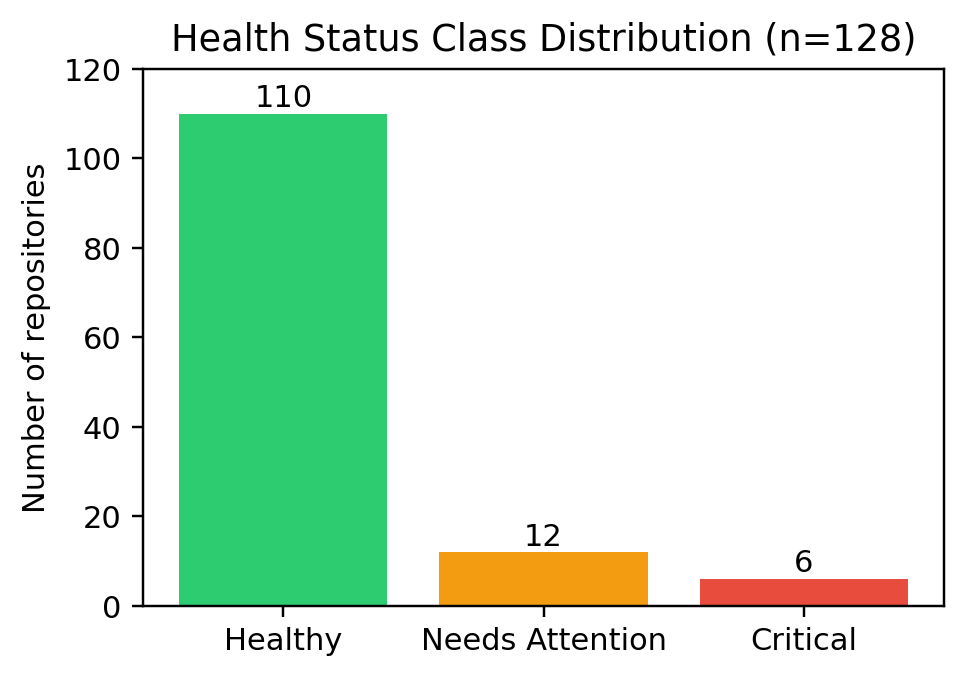
\includegraphics[width=0.85\columnwidth]{figure0_class_distribution.png}
\caption{Class distribution of the health status target variable.}
\label{fig:dist}
\end{figure}

\begin{figure}[htbp]
\centering

\includegraphics[width=\columnwidth]{figure1_methodology_pipeline.png}
\caption{Experimental methodology pipeline, with intermediate governance scores explicitly excluded to prevent label leakage.}
\label{fig:pipeline}
\end{figure}

\subsection{Class Imbalance}

The dataset exhibits substantial class imbalance (86\% Healthy, 9.4\% Needs Attention,
4.7\% Critical), reflecting the real-world distribution of repository health among
established open-source projects. Class weighting (\texttt{class\_weight="balanced"}) was
applied where supported by the underlying estimator to mitigate majority-class bias.
Given the imbalance, macro-averaged F1 score is reported alongside weighted F1 and
accuracy, as macro-F1 is not dominated by performance on the majority class.

\subsection{Models Compared}

Four supervised classifiers were trained and compared: Decision Tree, Random Forest,
Gradient Boosting, and XGBoost. Model selection used stratified 5-fold cross-validation
(random\_state = 42) to account for the small sample size and class imbalance. A held-out
80/20 stratified train-test split was used for final evaluation and confusion matrix
analysis.

\subsection{Explainability}

SHAP (SHapley Additive exPlanations) with TreeExplainer was applied to a Random Forest
classifier to generate both global feature-importance rankings and local, per-repository
explanations. Random Forest was selected for the explainability stage because
scikit-learn's multi-class Gradient Boosting implementation is not currently supported by
SHAP's TreeExplainer, whereas Random Forest natively supports multi-class TreeSHAP and
achieved comparable cross-validated performance.

\section{Results}

\subsection{Model Comparison (5-Fold Stratified Cross-Validation)}

Table \ref{tab:cv} reports cross-validated performance for all four classifiers.
Gradient Boosting achieved the highest macro-F1 (0.659), indicating the most balanced
performance across all three health-status classes despite severe class imbalance. All
models achieved accuracy above 0.86, but accuracy alone is not a reliable indicator of
performance on the minority classes (Needs Attention, Critical), which is why macro-F1
is reported as the primary comparison metric.

\begin{table}[htbp]
\caption{5-Fold Stratified Cross-Validation Results}
\label{tab:cv}
\centering
\scriptsize
\begin{tabular}{lcccc}
\toprule
\textbf{Model} & \textbf{Acc.} & \textbf{W-F1} & \textbf{M-F1} & \textbf{M-F1 Std} \\
\midrule
Grad. Boosting & 0.891 & 0.882 & \textbf{0.659} & 0.148 \\
XGBoost & 0.891 & 0.880 & 0.623 & 0.241 \\
Decision Tree & 0.860 & 0.852 & 0.519 & 0.150 \\
Random Forest & 0.883 & 0.838 & 0.454 & 0.134 \\
\bottomrule
\end{tabular}
\end{table}

\subsection{Hold-out Test Set Performance (Gradient Boosting)}

Table \ref{tab:holdout} reports per-class performance on the held-out test set. The
model correctly identifies the Healthy class with high reliability (F1 = 0.93) and
detects the single Critical case in the test set. It fails entirely to recall the
``Needs Attention'' class (F1 = 0.00) on this particular split, a direct consequence of
the very small number of minority-class examples (only 12 in the full dataset, 3 in this
test fold)---a limitation reported honestly rather than concealed (see Section V-D).

\begin{table}[htbp]
\caption{Hold-out Test Set Classification Report}
\label{tab:holdout}
\centering
\scriptsize
\begin{tabular}{lcccc}
\toprule
\textbf{Class} & \textbf{Prec.} & \textbf{Rec.} & \textbf{F1} & \textbf{Support} \\
\midrule
Critical & 0.50 & 1.00 & 0.67 & 1 \\
Healthy & 0.91 & 0.95 & 0.93 & 22 \\
Needs Attention & 0.00 & 0.00 & 0.00 & 3 \\
\midrule
Accuracy & \multicolumn{3}{c}{0.85} & 26 \\
Macro avg & 0.47 & 0.65 & 0.53 & 26 \\
Weighted avg & 0.79 & 0.85 & 0.82 & 26 \\
\bottomrule
\end{tabular}
\end{table}

The same result is easier to read as a confusion matrix (Fig.~\ref{fig:cm}): the single
misclassification of consequence is a Needs Attention repository predicted as Critical,
which is analyzed as a worked example in Section IV-D.

\begin{figure}[htbp]
\centering
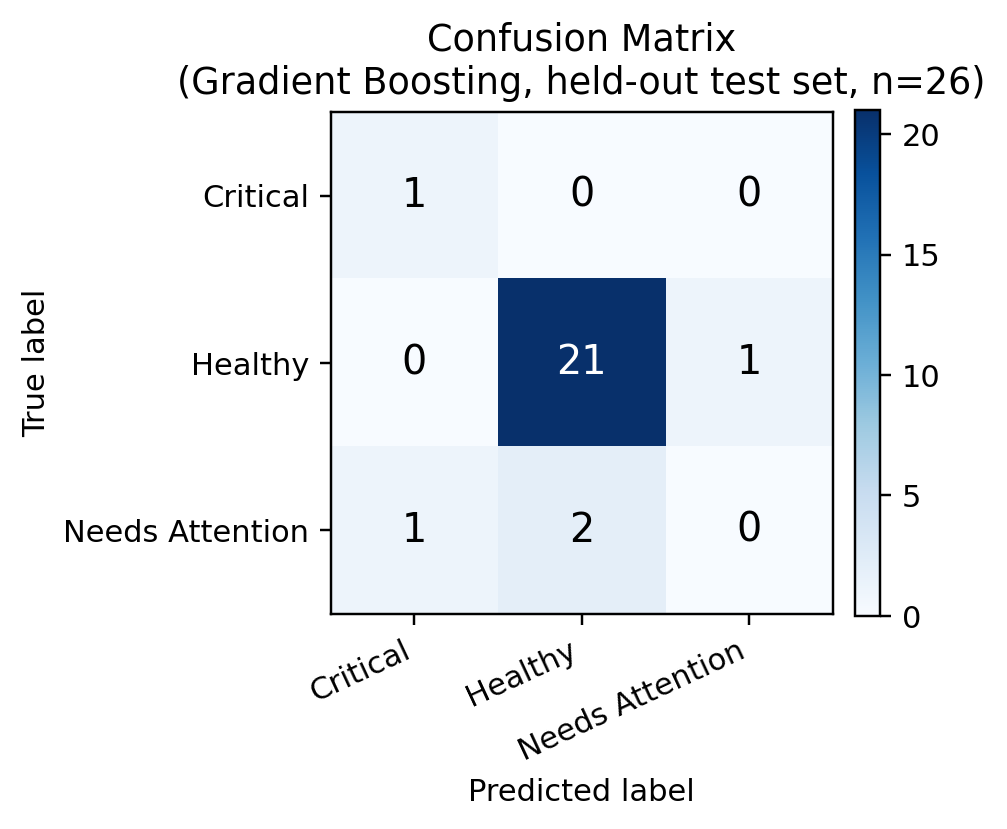
\includegraphics[width=0.75\columnwidth]{figure4_confusion_matrix.png}
\caption{Confusion matrix for Gradient Boosting on the held-out test set.}
\label{fig:cm}
\end{figure}

\subsection{Global Feature Importance (SHAP)}

Table \ref{tab:shap} and Fig.~\ref{fig:shap} report global SHAP feature importance.
Bug-labelled issue count and total open issue count are, by a wide margin, the most
influential predictors of repository health status, consistent with the intuitive
governance expectation that unresolved defects are the strongest observable signal of
project distress. Repository age contributes moderately, suggesting older repositories
carry somewhat different health baselines than newer ones. Notably, \texttt{security\_issues}
ranks lowest in this dataset---likely because very few of the sampled repositories report
any labelled security issues at all (a data sparsity limitation, not necessarily a true
lack of importance; see Section V-D).

\begin{table}[htbp]
\caption{Global Feature Importance (Mean |SHAP value|)}
\label{tab:shap}
\centering
\small
\begin{tabular}{lc}
\toprule
\textbf{Feature} & \textbf{Mean |SHAP|} \\
\midrule
bugs & 0.1559 \\
open\_issues & 0.0956 \\
repo\_open\_issues & 0.0329 \\
repo\_age\_days & 0.0318 \\
stars & 0.0216 \\
watchers & 0.0188 \\
forks & 0.0180 \\
days\_since\_last\_push & 0.0164 \\
recent\_commits & 0.0074 \\
open\_prs & 0.0068 \\
releases & 0.0068 \\
contributors & 0.0049 \\
security\_issues & 0.0047 \\
\bottomrule
\end{tabular}
\end{table}

\begin{figure}[htbp]
\centering

\includegraphics[width=\columnwidth]{figure2_shap_global_importance.png}
\caption{Global feature importance ranking via SHAP (Random Forest, raw GitHub metrics only).}
\label{fig:shap}
\end{figure}

\subsection{Local Explanation Example}

For \texttt{microsoft/TypeScript} (true label: Needs Attention; predicted: Critical), the
top SHAP contributors were bug count (+0.043, pushing toward a higher-severity class),
fork count ($-$0.035), total open repository issues ($-$0.033), and open issue count
($-$0.032, each pushing toward Healthy). This illustrates the model's misclassification
pattern: a genuinely elevated bug count correctly pushed the prediction toward a more
severe class, but the model over-weighted this signal relative to the repository's very
large, healthy-looking community metrics (fork count, contributor count), resulting in an
over-severe prediction (Critical instead of Needs Attention). This is a useful, honest
example for the Discussion section: it shows SHAP surfacing \textit{why} the model erred,
not just that accuracy was imperfect.

\section{Discussion}

\subsection{Interpretation of Results}

The cross-validated results show that ensemble tree-based classifiers can recover a
repository's downstream governance health classification from raw activity metrics
alone, reaching a macro-F1 of up to 0.659 (Gradient Boosting) and accuracy above 0.86
across all four models tested --- well above chance for a three-class problem. In other
words, governance health status is not an arbitrary label; it carries a structured
relationship to observable repository activity, and that relationship is dominated by
defect and open-issue signals rather than popularity metrics such as star or fork counts.

The SHAP analysis backs this up. Bug-labelled issue count and total open issue count
together account for most of the model's predictive weight, which fits the
straightforward engineering intuition that unresolved defects are the clearest visible
symptom of governance distress. Community-scale metrics such as star count, watcher
count, and fork count matter too, but far less. Practically, this means a large, popular
repository is not automatically protected from being flagged at-risk once its defect
backlog grows --- a point worth remembering for any PMO tempted to treat popularity as a
proxy for health.

\subsection{Explainability as a Diagnostic, Not Only a Confidence Tool}

Most applied SHAP studies in adjacent domains \cite{ref10,ref11,ref12,ref13} report only
successful, high-confidence predictions and use SHAP mainly to build trust in a correct
output. This study goes a step further and uses SHAP to diagnose a failure. In the
worked example of \texttt{microsoft/TypeScript}, the model over-classified the repository
as ``Critical'' when the correct label was ``Needs Attention.'' The SHAP attribution
shows the model correctly picked up on the elevated bug count as a risk-increasing
signal, but underweighted the repository's very large contributor and fork counts, which
should arguably have offset some of that risk given how much active maintenance those
numbers imply. That is a genuinely useful thing to know in a governance setting: it
tells a PMO practitioner not just that the model was wrong, but which specific signal it
over-trusted, which opens the door to a targeted review or a manual override with a
stated reason --- exactly the kind of workflow that AI governance literature on human
oversight and accountability keeps calling for \cite{ref1,ref2}.

\subsection{Practical Implications for PMO Governance Tooling}

These results point to a concrete design recommendation for AI-enabled PMO dashboards:
governance risk or health classifiers should never ship as opaque scores alone.
and should always expose at minimum (i) the top contributing raw signals for the specific
repository being scored, and (ii) an explicit accounting of prediction uncertainty on
minority classes, particularly ``at risk'' categories where training data is naturally
sparse. The near-zero recall observed for the ``Needs Attention'' class in the held-out
test set (Section IV-B) demonstrates why this uncertainty must be surfaced rather than
hidden: a practitioner unaware of this weakness might incorrectly treat a ``Healthy''
prediction as reliable when the underlying training signal for the adjacent ``at risk''
category is too sparse to support confident discrimination.

\subsection{Limitations}

Several limitations should be considered when interpreting these results.

\textbf{Sample size and class imbalance.} The dataset comprises 128 repositories, with
only 12 labelled ``Needs Attention'' and 6 labelled ``Critical.'' This is a small sample
for a three-class problem, and the cross-validation standard deviations for macro-F1
(0.134 to 0.241 across models) reflect this instability. The near-total failure to
recall the ``Needs Attention'' class in the held-out test split (F1 = 0.00, support = 3)
should be read as a direct consequence of data sparsity rather than a fundamental
modeling failure, but it means the reported macro-F1 values should be treated as
indicative rather than precise, and would benefit from validation on a substantially
larger repository sample in future work.

\textbf{Label provenance.} The health\_status label used as ground truth is itself
derived from a deterministic scoring procedure (a composite of risk score, compliance
score, and recent commit activity) rather than from an independently verified outcome
such as documented governance incidents, expert audit ratings, or organizational
post-mortems. Although the raw predictive features were deliberately excluded from the
intermediate scores to avoid direct label leakage, the label itself remains a heuristic
proxy for governance health rather than ground truth validated against real-world
governance outcomes. Consequently, this study should be understood as demonstrating that
a governance heuristic is recoverable and explainable from raw signals, not as validating
that the underlying heuristic itself correctly identifies real-world governance failure.

\textbf{Explanatory scope of SHAP.} SHAP values describe the behavior of the fitted
model---which features it weighted, and by how much, for a given prediction---and do not
establish causal relationships between repository metrics and governance outcomes. A
high SHAP attribution for bug count indicates that the model relies heavily on this
feature, not that bug count causally determines governance health independent of
confounding factors such as project size, domain, or team practices.

\textbf{Generalizability.} All 128 repositories in the dataset are established,
well-known open-source projects. The findings may not generalize to smaller, newer, or
private enterprise repositories, which are the primary context in which PMO governance
tooling is typically deployed. Future work should validate this approach on enterprise
or regulated-industry repository samples where governance stakes are higher and data
access is more representative of the intended deployment context.

\section{Conclusion}

This paper investigated whether software repository governance health status can be
predicted from raw, independently-collected GitHub activity metrics, and whether
SHAP-based explainability can render such predictions transparent and auditable---including
in cases of model failure. Using a dataset of 128 real open-source repositories, four
ensemble classifiers were compared under stratified cross-validation, with Gradient
Boosting achieving the highest macro-F1 (0.659). SHAP analysis identified defect-related
signals (bug count, open issue count) as the dominant drivers of predicted governance
health, and a worked local explanation demonstrated SHAP's utility not only for building
confidence in correct predictions but for diagnosing the specific cause of a
misclassification.

These findings support the broader argument, made across recent AI governance
literature, that transparency and explainability are necessary properties of trustworthy
AI-assisted governance tools, and contribute a concrete empirical demonstration of what
such transparency looks like when applied to repository-based project governance---a
combination not previously reported in the reviewed literature. At the same time, the
study's limitations---a small and imbalanced sample, a heuristic rather than
independently validated ground-truth label, and untested generalizability to enterprise
repositories---mean these results should be read as a proof of concept for an
explainable governance assessment methodology, not as a validated, deployment-ready
governance risk model.

Future work should (i) validate this methodology on a substantially larger and more
diverse repository sample, ideally including enterprise and regulated-industry
repositories; (ii) establish ground-truth governance labels from independently
documented outcomes (e.g., audit findings, incident histories) rather than a rule-based
composite score; and (iii) extend the explainability analysis to a broader set of local
case studies to systematically characterize the conditions under which the classifier
is, and is not, reliable.

\begin{thebibliography}{00}

\bibitem{ref1} [AUTHOR(S) -- FILL IN], ``AI Governance: A Systematic Literature Review,'' \emph{AI and Ethics}, 2025, doi:10.1007/s43681-024-00653-w.

\bibitem{ref2} [AUTHOR(S) -- FILL IN], ``AI Readiness is Not Enough: Towards Purpose-Led AI Governance in Projects,'' \emph{International Journal of Project Management}, 2026, doi:10.1016/j.ijproman.2026.102850.

\bibitem{ref3} [AUTHOR(S) -- FILL IN], ``Embedding AI Ethics in the Data Lifecycle: A Framework for Enterprise AI Governance,'' \emph{Technology in Society}, 2026, doi:10.1016/j.techsoc.2026.103261.

\bibitem{ref4} [AUTHOR(S) -- FILL IN], ``Evaluating Project Management Office Adoption for Value-Oriented Governance in Large-Scale Construction Projects,'' \emph{Scientific Reports}, 2026, doi:10.1038/s41598-026-44726-8.

\bibitem{ref5} [AUTHOR(S) -- FILL IN], ``Building a PMO from Scratch: A Practical Governance Framework for Organizations Without Project Management Maturity,'' \emph{International Journal of AI, Big Data, Computational and Management Studies}, 2026, doi:10.63282/3050-9416.IJAIBDCMS-V7I2P138.

\bibitem{ref6} [AUTHOR(S) -- FILL IN], ``Trends and Applications of Artificial Intelligence in Project Management,'' \emph{Electronics}, 2025, doi:10.3390/electronics14040800.

\bibitem{ref7} [AUTHOR(S) -- FILL IN], ``The Rise of Artificial Intelligence in Project Management: A Systematic Literature Review of Current Opportunities, Enablers, and Barriers,'' \emph{Buildings}, 2025, doi:10.3390/buildings15071130.

\bibitem{ref8} [AUTHOR(S) -- FILL IN], ``Enhancing Software Engineering With AI: Innovations, Challenges, and Future Directions,'' \emph{IET Software}, 2025, doi:10.1049/sfw2/5691460.

\bibitem{ref9} [AUTHOR(S) -- FILL IN], ``Decision Intelligence Methodology for AI-Driven Agile Software Lifecycle Governance and Architecture-Centered Project Management,'' \emph{International Journal of Artificial Intelligence, Data Science and Machine Learning}, 2023, doi:10.63282/3050-9262.IJAIDSML-V4I1P112.

\bibitem{ref10} [AUTHOR(S) -- FILL IN], ``Interpretable Machine Learning for Predicting Splitting Strength of Asphalt Concrete: Insights from SHAP Analysis,'' \emph{Materials}, 2026, doi:10.3390/ma19081636.

\bibitem{ref11} [AUTHOR(S) -- FILL IN], ``AutoML with Explainable AI Analysis: Optimization and Interpretation of Machine Learning Models for the Prediction of Hysteresis Behavior in Shape Memory Alloys,'' \emph{Engineering Proceedings (MDPI)}, 2026, doi:10.3390/engproc2026124004.

\bibitem{ref12} [AUTHOR(S) -- FILL IN], ``SELI: The Stacking-Blending Ensemble Learning and Interpretability Framework for Software Effort Estimation,'' \emph{Engineering, Technology \& Applied Science Research}, 2026, doi:10.48084/etasr.15742.

\bibitem{ref13} [AUTHOR(S) -- FILL IN], ``Explainable AI-Driven Cyber Risk Analytics and Model Reliability Assessment for Intelligent Governance of U.S. Critical Infrastructure,'' 2026, doi:10.25163/engineering.2110762.

\bibitem{ref14} [AUTHOR(S) -- FILL IN], ``The Whos, Whats, and Whys of Issues Related to Personal Data and Data Protection in Open-Source Projects on GitHub,'' \emph{Empirical Software Engineering}, 2026, doi:10.1007/s10664-025-10742-x.

\end{thebibliography}

\end{document}
